% Efeito da temperatura na distribuição do token seguinte (valores ilustrativos)
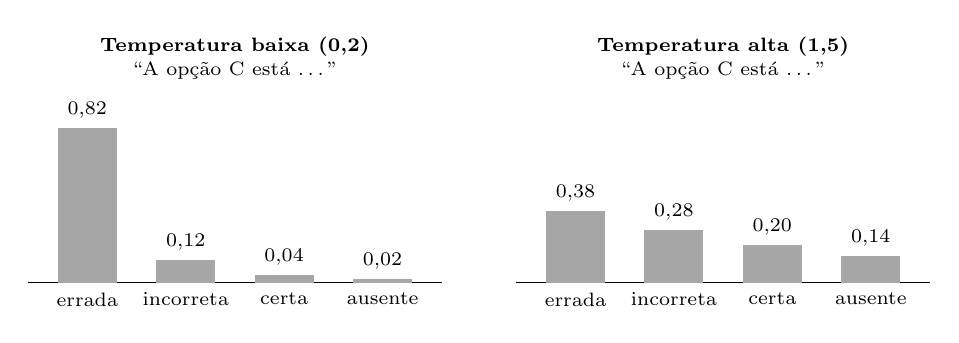
\begin{tikzpicture}[x=1.25cm, y=2.4cm, lab/.style={font=\scriptsize}]
\foreach \dx/\titulo/\vals in {0/{Temperatura baixa (0,2)}/{0.82/{0,82},0.12/{0,12},0.04/{0,04},0.02/{0,02}}, 6.2/{Temperatura alta (1,5)}/{0.38/{0,38},0.28/{0,28},0.20/{0,20},0.14/{0,14}}} {
  \begin{scope}[xshift=\dx cm]
    \node[lab, font=\scriptsize\bfseries] at (2,1.25) {\titulo};
    \node[lab] at (2,1.12) {``A opção C está \dots''};
    \draw (-0.1,0) -- (4.1,0);
    \foreach [count=\i] \v/\t in \vals {
      \fill[black!35] (\i-0.8,0) rectangle (\i-0.2,\v);
      \node[lab, above] at (\i-0.5,\v) {\t};
    }
    \foreach [count=\i] \w in {errada, incorreta, certa, ausente}
      \node[lab, below] at (\i-0.5,0) {\w};
  \end{scope}
}
\end{tikzpicture}
